\chapter{}
\chapter{}
\chapter{}

\section{Chap. 3 Exercices, série 1 }

\subsection{Exercice: Incertitudes des appareils }
Spécifications:\\
\\
\textbf{HP34401A}: spécifié pour 1 an, $23 \pm 5 \degree C$, en (\%lect+ \%gamme) et jusqu'à 20\% de dépassement de gamme\\
\\
\begin{tabular}{l c c}
    \hline
    gamme: & 100.0000 mV & 0.0050 + 0.0035 \\
           & 1.000000 V  & 0.0040 + 0.0007 \\
           & 10.00000 V  & 0.0035 + 0.0005 \\
           & 100.0000 V  & 0.0045 + 0.0006 \\
           & 1000.000 V  & 0.0045 + 0.0010 \\
    \hline
\end{tabular}
\\
\\
\textbf{Prema} 6000:spécifs pour 1 an, $23 \pm 5 \degree C$, en (\% of reading + \% of full scale)
Full scale : 1'999'999 (sauf gamme 1000 V : 1'000'000)
\\
\begin{tabular}{lcc}
    \hline
    range & $\pm$ 0.2 V  & 0.006 + 0.0007 \\
          & $\pm$ 2 V    & 0.005 + 0.0005 \\
          & $\pm$ 20 V   & 0.005 + 0.0006 \\
          & $\pm$ 200 V  & 0.005 + 0.0006 \\
          & $\pm$ 1000 V & 0.006 + 0.0005 \\
    \hline
\end{tabular}
\\
\\
\textbf{APPA-98}: spécifié pour 2 ans, $23 \pm 5 \degree C$ et moins de 75\% humidité relative, en (\% reading + number of digits)
\\
\begin{tabular}{lcl}
    \hline
    Range  & Resolution & Accuracy                     \\
    200 mV & 100 $\mu$V & |                            \\
    2 V    & 1 mV       & |                            \\
    20 V   & 10 mV      & |  $\pm$ (0.5 \%rdg + 1 dgt) \\
    200 V  & 100 mV     & |                            \\
    1000 V & 1 V        & |                            \\
    \hline
\end{tabular}
\\

\begin{enumerate}
    \item Quelles sont les incertitudes absolues et relatives si on mesure 2.2 V avec HP34401A ?
    \item Quelles sont les incertitudes absolues et relatives si on mesure 2.2 V avec APPA-98 ?
    \item Quelle est l'incertitude relative maximum si on mesure entre 10 et 250 mV avec HP34401A ?
    \item Quelle est l'incertitude relative maximum si on mesure entre 10 et 250 mV avec Prema6000 ?
    \item Quelle est l'incertitude absolue maximum si l'on mesure entre 30 et 500 V avec APPA-98 ?
    \item Représenter les incertitudes relatives du HP34401A et du Prema6000 pour un domaine de 10mV à 1000V (utilisez une échelle Log pour l'axe X des tensions).
\end{enumerate}
NB: la pleine échelle définie pour le PREMA n'est pas la définition habituelle qui dit que la pleine échelle est la différence entre les valeurs min et max. On aurait alors attendu pour le PREMA une pleine échelle égale au double de la gamme.

\subsection{Exercice: Ajustage d'une chaîne}
a)	Une chaîne de mesure de température doit être utilisée pour la régulation de température d'une enceinte, autour de 60 $\degree$ C. On désire qu'elle nous indique l'erreur (température actuelle moins consigne de 60 $\degree$ C). L'ajustage est réalisé ainsi: \\
i)	on place le capteur dans un bain à 60 $\pm$ 0.35 $\degree$ C, et on ajuste le décalage pour un affichage nominal de 0.00. On constate que les indications oscillent entre -0.03 et + 0.08. \\
ii)	on place le capteur dans un bain à 70 $\pm$ 0.5 $\degree$ C, et on ajuste le gain pour un affichage nominal de 10.00. On constate que les indications oscillent entre 9.88 et 10.09. \\  ~ \\
Quelles sont les incertitudes de gain et de décalage dues à cet ajustage ? \\

b)	Une chaîne de mesure doit indiquer l'épaisseur d'une feuille plastic (capteur capacitif sans contact, basé sur la variation de la constante diélectrique). L'ajustage s'effectue comme suit: \\
i)	Pas de feuille dans le capteur, on ajuste le décalage et on obtient un affichage stable de 000. \\
ii)	On place une feuille étalon d'épaisseur 0.500  $\pm$  0.005 mm dans le capteur, et on ajuste le gain pour un affichage nominal de 500. Malheureusement le potentiomètre ne permet pas l'ajustage exact et on doit se contenter d'un affichage oscillant entre 497 et 499. \\~ \\
Quelles sont les incertitudes d'ajustage de cette chaîne ? \\

c)	Une chaîne de mesure de la hauteur du liquide contenu dans un réservoir utilise la pression relative à la base de ce réservoir (P = $\rho\,gh$ où h est la hauteur du liquide dans le réservoir). Pour l'ajustage on procède comme suit: \\
i)	Réservoir vide, on ajuste le décalage pour un affichage de 0000  $\pm$  0001 \\
ii)	On remplit le réservoir, on mesure une hauteur h = 10.00 $\pm$ 0.02 m, ainsi que la densité du liquide  $\rho$ = 0.800  $\pm$  0.006 kg/dm3, et on ajuste l'affichage à 1000  $\pm$  0003 \\ ~ \\
Quelles sont les incertitudes d'ajustage (indication: n'oubliez pas que la chaîne est sensible à la pression et non directement à la hauteur du liquide)? \\

d)	On a calibré un capteur de pression relative (=différence de pression par rapport à l'atmosphère) de la manière suivante : pression appliquée par une pompe dans la tuyauterie du capteur avec une vanne de détente, mesure de la pression appliquée par la différence de hauteur de mercure dans un tube en U, ouvert sur l'atmosphère, lecture de la sortie dans un PC. La réponse nominale est 0 à +2 bar, 0 à +20'000digit (1 bar = 100kPa). \\
i)	Vanne ouverte (= pression atmosphérique), ajustage de l'offset pour une valeur nominale de 0, on obtient un affichage stable de 00'000digit. \\
ii)	Vanne fermée, on agit sur la pompe jusqu'à une hauteur de mercure de 148.5 $\pm$ 0.2cm dans le tube en U. On calcule alors la pression appliquée $P=\rho\,gh = 13.6\times10^3 \text{ kg/m}^3 * 9.81\text {m/s}^2 * 1.485\text{ m}=198.12276\text{ kPa} = 1.98123\text{ bar}$. On ajuste donc le gain pour obtenir un affichage nominal de 19'812.3 digit, et obtient un affichage oscillant entre 19'810 et 19'814. \\ ~\\
Quelles sont les incertitudes d'ajustage ?

\subsection{Exercice: Linéarité}

a)On a mesuré la réponse d'un capteur de force à $23 \degree C$ (réponse idéale : $0-100N \Leftrightarrow 0-20 mV$):\\
~
\\
\begin{tabular}{|l|l|l|l|l|l|l|l|l|l|l|l|}
    \hline
    F [N]  & 0    & 10   & 20   & 30   & 40   & 50    & 60    & 70    & 80    & 90    & 100  \\
    \hline
    U [mV] & 0.50 & 2.49 & 4.46 & 6.41 & 8.34 & 10.25 & 12.14 & 14.01 & 15.86 & 17.69 & 19.5 \\
    \hline
\end{tabular}
\\

Déterminez l'offset réel en [mV], le gain réel en [mV/N], les erreurs de décalage [N], de gain [\%lect] et l'incertitude de non-linéarité en [N] et en [\%(PE)] de ce montage par les deux méthodes :
\begin{enumerate}
    \item Choix de la droite de référence par les extrémités de la courbe de réponse
    \item Choix de la "meilleure droite"	 ...
\end{enumerate}
~\\

b)	L'étalonnage d'une chaîne de mesure de couple, gamme 0 à 100 mNm, sortie 4 à 20 mA, a donné: \\
~
\\
\begin{tabular}{|l|l|l|l|l|l|l|l|l|l|l|l|}
    \hline
    \footnotesize C [mNm] & 0                    & 10                   & 20                   & 30                   & 40                    & 50                    & 60                    & 70                    & 80                    & 90                    & 100                   \\
    \hline

    \footnotesize I [mA]  & \footnotesize  3.960 & \footnotesize  5.564 & \footnotesize  7.192 & \footnotesize  8.800 & \footnotesize  10.443 & \footnotesize  12.063 & \footnotesize  13.677 & \footnotesize  15.315 & \footnotesize  16.926 & \footnotesize  18.550 & \footnotesize  20.160 \\
    \hline
\end{tabular}
\\

L'équation nominale de cette chaîne vaut donc $I = 4 [mA] + 0.16 [\frac{mA}{mNm}]  \cdot C [mNm]$.

Quelles sont les erreurs de gain et de décalage ainsi que l'incertitude de non-linéraité + bruit dans les 2 cas suivants:
\begin{enumerate}
    \item Choix de la droite de référence par les extrémités de la courbe de réponse
    \item Choix de la "meilleure droite"	 ...
\end{enumerate}

\subsection{Exercice: Auto-Calibrage d'une chaîne}

a)	Pour réaliser l'auto-calibrage d'un canal de mesure de courant (nominal 0-20 mA, code numériques 0-2000 digits), on procède comme suit:
\begin{itemize}
    \item ouverture du circuit de mesure par un interrupteur (donc courant nul), mémorisation du code obtenu :  $N_0=2$ (stable)
    \item Fermeture d'un interrupteur reliant une source de tension de référence ($U_g = 10.000V \pm 0.005V$) au circuit de mesure à travers une résistance de $R_g = 500 \Omega \pm 0.1\%$ (la borne de mesure étant supposée travailler à potentiel nul, le courant nominal ainsi imposé est de 20mA). On mémorise alors le code moyen obtenu sur 10 mesures : $N_1 = 2018.3$, alors que les codes max et min sont 2021 et 2015.
    \item Les mesures seront ensuite corrigées à l'aide de $N_0$ et $N_1$ pour obtenir :
          \begin{itemize}\itemsep1pt
                    \renewcommand{\labelitemi}{$\bullet$}
              \item i) une valeur numérique corrigée ;
              \item ii) une valeur dans l'unité du mesurande ;
          \end{itemize}
\end{itemize}
NB : si ces corrections sont faites à l'extérieur de la chaîne de mesure, alors on parlera d'auto-étalonnage.
Quelles sont les fonctions mathématiques de correction et quelles sont les incertitudes d'ajustage ?\\

b)	Pour programmer l'auto-calibrage d'une chaîne de mesure de température dont le capteur (PT100 : $R(T)=100 \Omega (1+0.00385T)$ a une interchangeabilité de 0.2 $\degree$ C + 0.1\%lecture, on a inséré des interrupteurs programmables permettant de déconnecter le capteur et de le remplacer soit par une résistance de$ 100 \Omega \pm 0.1 \Omega$, soit par une résistance de $138.5 \Omega \pm 0.14 \Omega$. La séquence d'auto-calibrage est la suivante :
\begin{itemize}
    \item Capteur remplacé par la résistance de $100 \Omega$, on mémorise la moyenne de 100 conversions: on trouve $M_0=1985.65$, toutes les conversions sont soit 1985, soit 1986.
    \item Capteur remplacé par la résistance de $138.5 \Omega$. On mémorise la moyenne de 100 conversions: $M_1=2825.45$, conversion maximum 2827, minimum 2824.
    \item Pour les mesures, on ne fait qu'une seule conversion $N_x$, et l'on calcule \\
          $T= (N_x - M_0)\frac{100}{M_1 - M_0}$
\end{itemize}
Quelles sont les incertitudes d'ajustage ? \\

c)	Une chaîne de mesure de pression est constituée d'un capteur-transmetteur avec les spécifications suivantes : gamme -1 à +3 bar, sortie 4 à 20mA, précision 0.5\%lect + 35 mbar ; le courant de sortie est mesuré par une résistance shunt de $10 \Omega \pm 0.012 \Omega$, et un convertisseur gamme $\pm 0.25V$.
Pour programmer l'auto-calibrage de cette chaîne, on a inséré des interrupteurs programmables permettant de déconnecter le capteur et de le remplacer soit en laissant le circuit ouvert, soit en reliant une résistance de $490 \Omega \pm 0.2 \Omega$ entre la borne positive du shunt et une source de tension de $+10V \pm 15mV$ (courant nominal de 20 mA). La séquence d'auto-calibrage est la suivante :
\begin{itemize}
    \item Capteur déconnecté, circuit ouvert on mémorise la moyenne de 100 conversions: on trouve $M_0=-0.73$ digit, toutes les conversions sont soit -1, soit 0 digit.
    \item Capteur déconnecté, résistance $490 \Omega$ enclenchée. On mémorise la moyenne de 100 conversions: $M_1=1647.32$, conversion maximum 1646, minimum 1649 digit.
    \item Les valeurs de $M_0$ et $M_1$ nous permettent de calculer le gain et l'offset total actuel de la chaîne.
\end{itemize}

Quelles sont les incertitudes d'ajustage ?

\subsection{Exercice: Coefficients d'influence}

a)	On a étalonné une chaîne de mesure de position à deux températures:


\begin {center}
\begin{tabular}{lll}
    $T_1=25 \degree C$ & $G_1= 100.3 digit/mm$  & $Of_1 = 3.4 digit$  \\
    $T_2=75 \degree C$ & $G_2 = 103.5 digit/mm$ & $Of_2 = -5.8 digit$ \\
\end{tabular}
\end{center}
~\\
\begin{itemize}
    \item Déterminer les coefficients d'influence de la température
    \item A une température de 40 $\degree$ C, l'indication obtenue est de 1380 digit. Calculer la position correspondante
\end{itemize}
~\\


b)	Une chaîne de mesure du contenu d'un réservoir utilise un capteur de force à jauges de contraintes (pont de Wheatstone à 4 jauges)

\begin{figure}[h!]
    \centering
    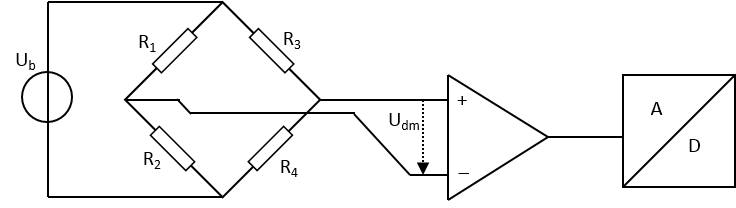
\includegraphics[height=3.7cm]{assets/figures/Exercice_3_5_c.PNG}
    \caption{Chaîne de mesure du contenu d'un réservoir.}
    \label{fig:Exercice_3_5_c}
\end{figure}

\begin{center}
    $R_1 = R_4 = R_0(1 + F \cdot K)$\\
    $R_2 = R_3 = R_0(1 - F \cdot K)$\\
\end{center}

Avec K = facteur de jauge et F = force appliquée.\\

On en déduit :	$U_{dm} = U_b ( \frac{ R_4}{R_3+R4} - \frac{R2}{R1+R2} ) = U_b \frac{ Ro(1+KF) -Ro(1-KF)}{2Ro}  = Ub \cdot K \cdot F$ \\
La sortie est donc théoriquement proportionnelle à la force, mais aussi à la tension d'alimentation $U_b$, on parle alors de capteur ratio-métrique : la sortie est une fraction (ratio) de l'alimentation.

On a étalonné la chaîne dans les 3 conditions suivantes :\\

\begin {center}
\begin{tabular}{llll}
    $U_b = 5V$ & $T=25 \degree C$ & $G_1 = 1015 digit/tonne$ & $Of_1 = -55 digit$ \\
    $U_b = 3V$ & $T=25 \degree C$ & $G_2 = 609 digit/tonne$  & $Of_2 = -33 digit$ \\
    $U_b = 5V$ & $T=50 \degree C$ & $G_3 = 1095 digit/tonne$ & $Of_3 = +12 digit$ \\
\end{tabular}
\end{center}
~\\
On suppose les influences indépendantes et linéaires

\begin{itemize}
    \item Calculer les coefficients d'influence de la température T et de l'alimentation $U_b$.
    \item Calculez le gain et l'offset pour une température $T=30 \degree C$ et une alimentation $U_b=5.5V$
    \item Enumérez les coefficients du moteur de correction IEEE1451
\end{itemize}

\subsection{Exercice: Mesures répétées}

Un expérimentateur utilise un capteur de pression différentielle dont on lui a dit que la plage de précision était de $\pm 2\%$, pour une différence de pression de 20 Pa, pour un intervalle de confiance de 95\%. Afin de vérifier cette affirmation, il étalonne le capteur en effectuant 100 mesures de la tension U donnée par le capteur lorsque la pression différentielle est p = 20 Pa (il contrôle cette pression de façon très précise). À partir de son échantillon de 100 mesures, il calcule $\mu = 5V$ et $\sigma = 0.2 V$. Il prétend que le capteur n'est pas aussi précis qu'on le lui avait certifié. Pourquoi?

